\section{Simulation Analysis}
\label{sec:simulation}

In this section we will be describing the simulation that we made on a software called NGSpice where we made a script describing the given circuit. After running the script, NGSpice gives us the variables that we are looking for, these variables are the same as the ones we calculated using both the mesh and nodal methods.

\subsection{NGSpice Simulation}

Firstly we’ve added the values for resistors, $V_a$, $I_d$, $K_b$ and $K_c$, from the python script and then we described the circuit based on the circuit below:

\begin{figure}[H] \centering
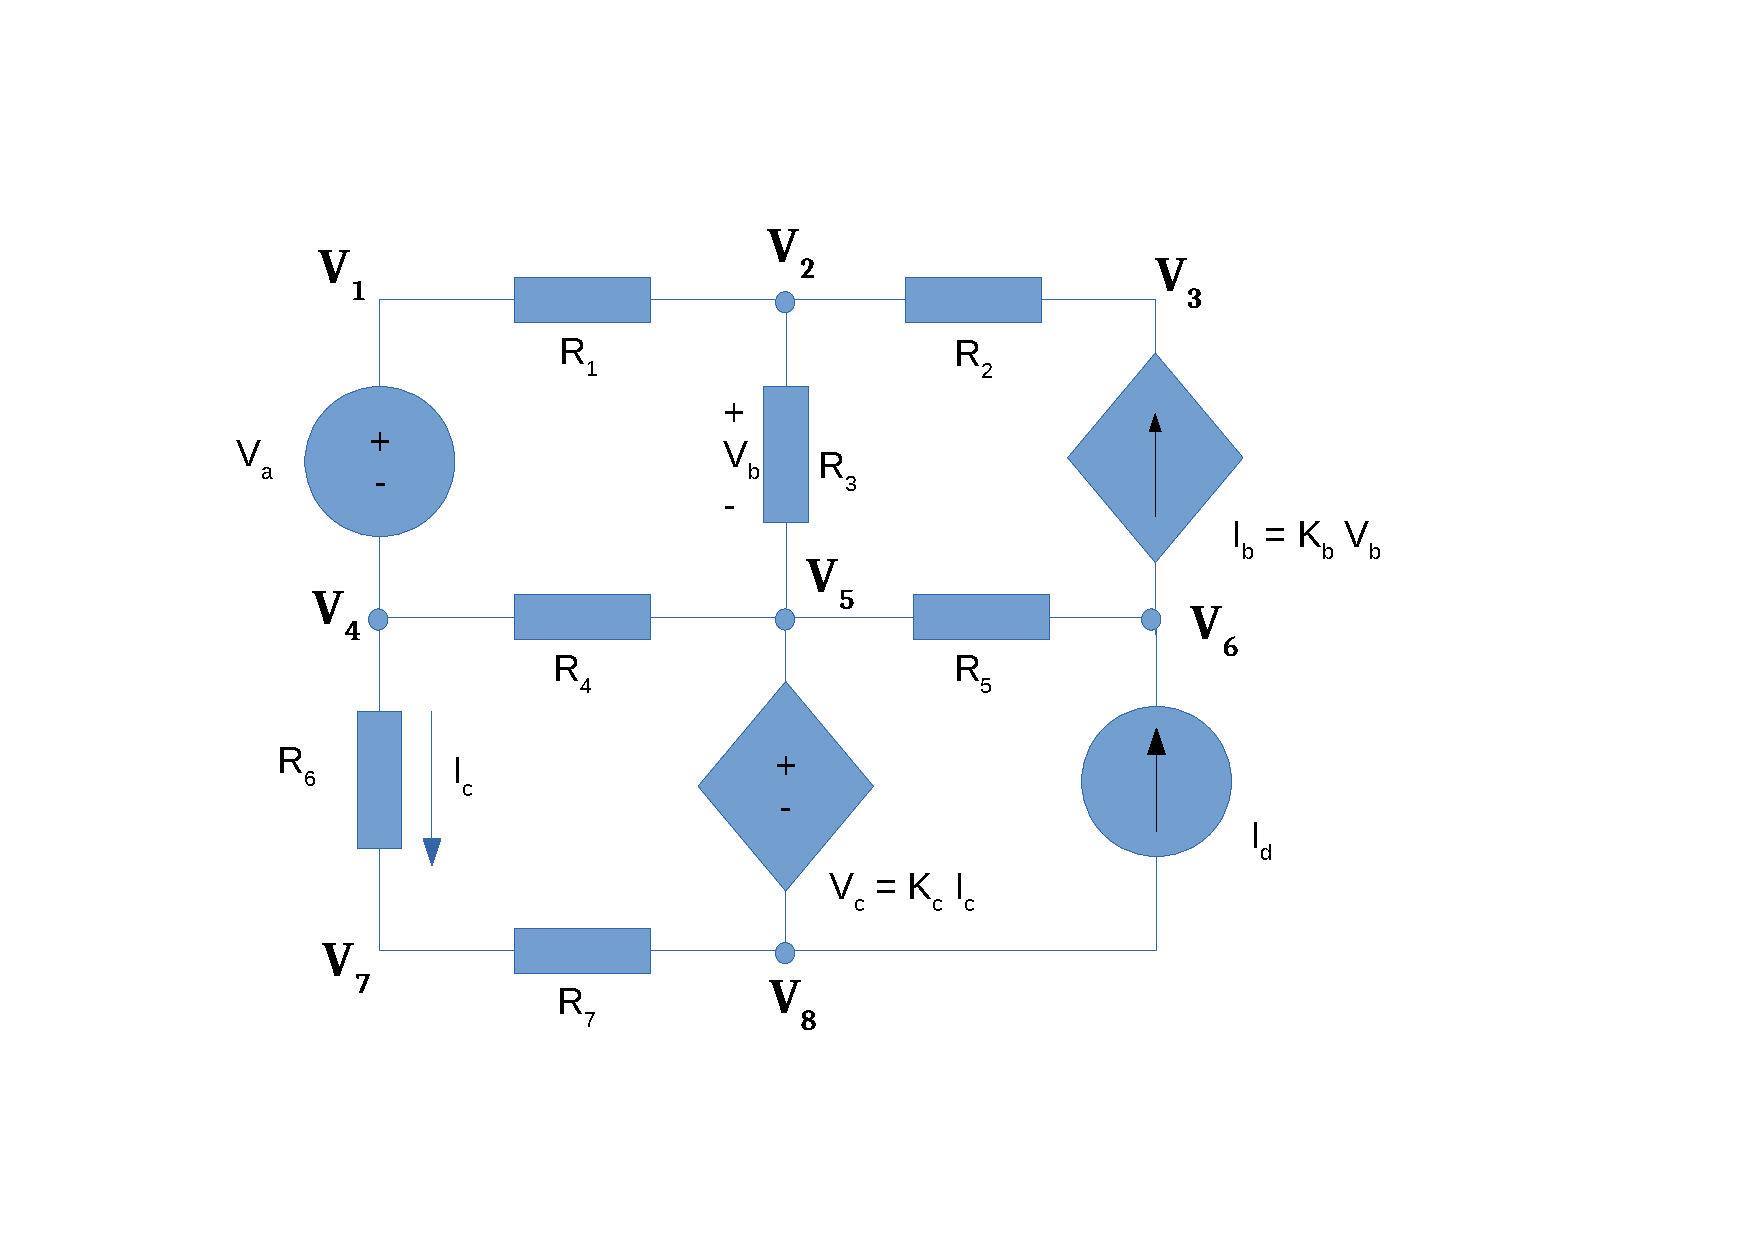
\includegraphics[width=0.7\linewidth]{ngspice.pdf}
\caption{NGSpice simulation circuit.}
\label{fig:ngspice}
\end{figure}


After running the script, the results we get using this simulation are organized in the table below.

\begin{table}[H]
  \centering
  \begin{tabular}{|l|r|}
    \hline    
    {\bf Name} & {\bf Value [A or V]} \\ \hline
    @g0[i] & -2.62010e-04\\ \hline
@id[current] & 1.039703e-03\\ \hline
@r1[i] & 2.500671e-04\\ \hline
@r2[i] & -2.62010e-04\\ \hline
@r3[i] & -1.19432e-05\\ \hline
@r4[i] & 1.159730e-03\\ \hline
@r5[i] & -1.30171e-03\\ \hline
@r6[i] & 9.096634e-04\\ \hline
@r7[i] & 9.096634e-04\\ \hline
n1 & 5.046111e+00\\ \hline
n2 & 4.787759e+00\\ \hline
n3 & 4.248290e+00\\ \hline
n4 & -1.88445e+00\\ \hline
n5 & 4.824275e+00\\ \hline
n6 & 8.832281e+00\\ \hline
n8 & -2.81232e+00\\ \hline
n9 & -1.88445e+00\\ \hline

  \end{tabular}
  \label{tab:op}
\end{table}

All the variables preceded by @ are currents and are expressed in Ampere, the other variables, preceeded by n are the voltages at each node and are expressed in Volt. \par
Using these voltages at the nodes, we can calculate the variables that were calculated above using both the mesh and nodal methods so we can compare them and see the what could be differences between them. \par

\begin{equation}
  V_b = n2 - n5 \quad \text{ which equals to } -0.036516V
  \label{eq18}
\end{equation}

\begin{equation}
  V_c = n8 - n5 \quad \text{ which equals to } -7.636595V
  \label{eq19}
\end{equation}

As for the currents $I_b$ and $I_c$, we can get them in the NGSpice results by seeing in which resistor the current is that value. $I_b$ is the current that goes through $R_2$ and therefore it is 0.262010$mA$ and $I_c$ is the current that goes through $R_6$ and therefore it is 0.9096634$mA$. \par
Putting these values in a table so that we can analyse them and compare them more easily we get the following table:

\begin{center}
  \begin{tabular}{ | c | c | }
    \hline    
    {\bf Name} & {\bf Value [A or V]} \\ \hline
    $V_b$ & -0.036516 \\ \hline 
    $V_c$ & -7.636595 \\ \hline 
    $I_b$ & 2.62010e-04 \\ \hline 
    $I_c$ & 9.096634e-04 \\ 
    \hline
  \end{tabular}
\end{center}

As we can see there are little differences in the last digit of some values. These differences are very small and can be explained with approximations that may have been used in some intermediate steps along the way, either by Octave or by NGSpice, or most probably both.


